\section{Stanowisko badawcze}
\label{sec:test_stand}

Konstrukcję stanowiska badawczego uzależniono od kilku czynników:
%lista punktowana
\begin{itemize}
\item prostota budowy
\item możliwość wymiany modelu przetwornika (patrz: Rys.\ref{fig:test_stand})
\item łatwa zmiana mocowania przetwornika
\item możliwość regulacji energii wymuszenia mechanicznego
\end{itemize}

\begin{figure}[htbp]
\centering
\fbox{TUTAJ PROJEKT STANOWISKA}%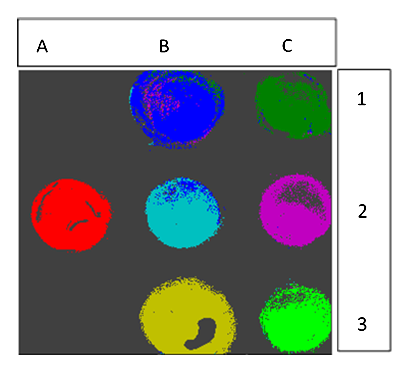
\includegraphics[width=\linewidth]{sample}}
\caption{Projekt stanowiska badawczego.}
\label{fig:test_stand}
\end{figure}

\begin{figure}[htbp]
\centering
\fbox{TUTAJ ZDJĘCIE STANOWISKA}%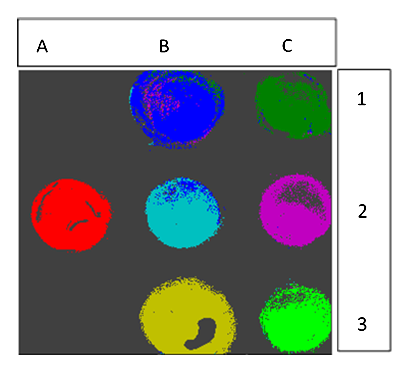
\includegraphics[width=\linewidth]{sample}}
\caption{Realizacja stanowiska badawczego.}
\label{fig:test_stand_photo}
\end{figure}